\documentclass[12pt,a4paper]{article}

\usepackage{mcode}
\usepackage{graphicx}
\usepackage{caption}
\usepackage{subcaption}

\lstset{language=Matlab}
\lstset{
  numbers=left,
  stepnumber=5,    
  firstnumber=1,
  numberfirstline=true
}

\begin{document}

\section{Scope of Simulation}



\section{Reference Frames}
There are 3 major reference frames that play a part in this system. 
\begin{enumerate}
\item Earth Centered Inertial frame (ECI)
\item Orbital Reference frame 
\item Body Centered frame
\end{enumerate}

\subsection{Earth Centered Inertial Frame}
The Earth Centered frame is the the frame of reference that shares its coordinate axis with the planet Earth. For the purpose of the simulation the ECI frame does not take into account the Earth's rotation; instead the frame $Z$ axis crosses both poles through the planet center. The $Y$ and $X$ axes are orthogonal, and make up the equatorial plane. For the purposes of initial conditions, the $X$ axis has been made to coincide with 0 degrees longitude ($0^{\circ}$ $0^{\circ}$). This value will change however as the Earth rotates with respect to the stationary frame. 

\begin{figure}[h!]
	\centering
	\begin{subfigure}[h!]{0.4\textwidth}
	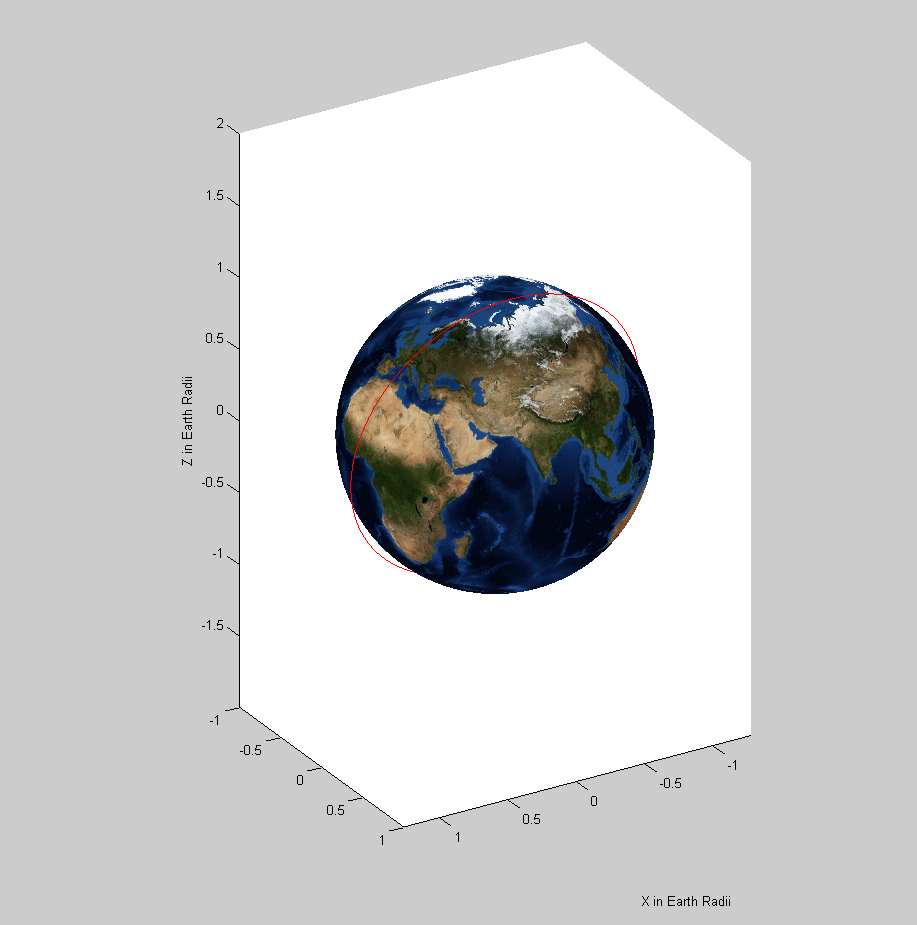
\includegraphics[scale=0.25]{ECI.png}
	\caption{The ECI frame of reference showing two orbital passes. Notice that the earth has not rotated underneath the orbiting satellite.}
	\end{subfigure}
	\hspace{2cm}
	\begin{subfigure}[h!]{0.4\textwidth}
	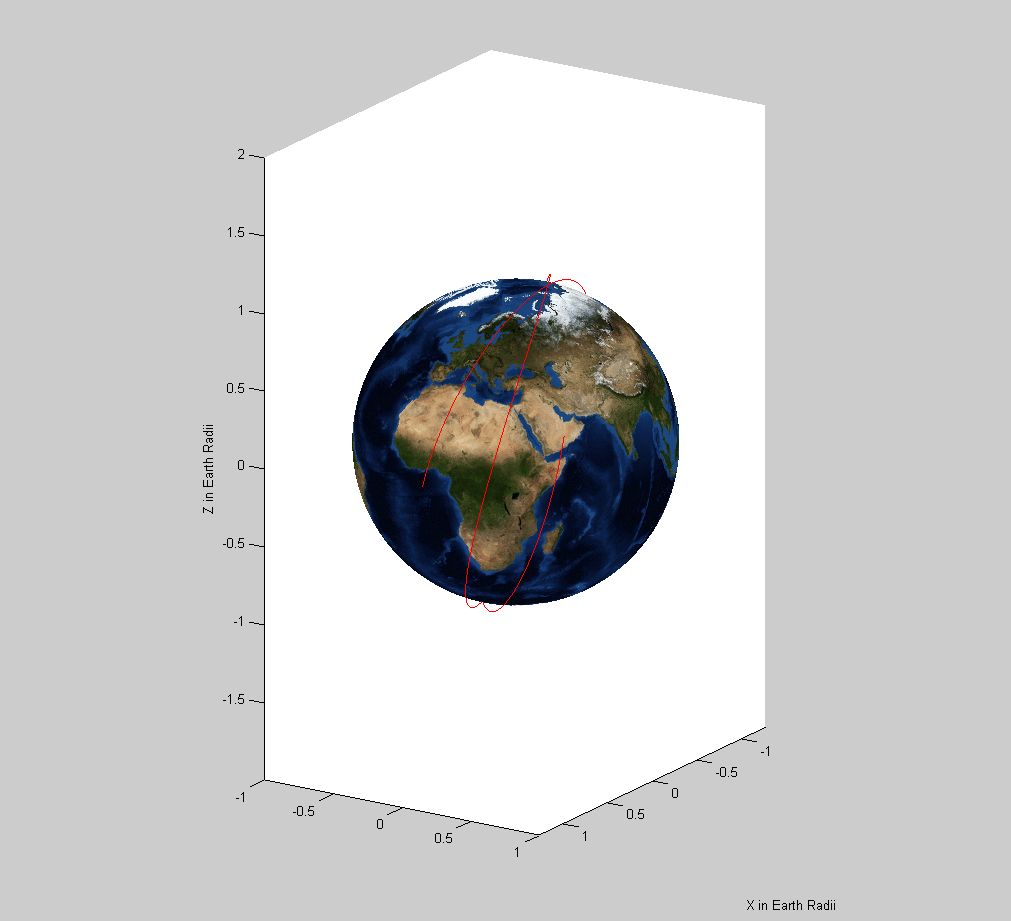
\includegraphics[scale=0.25]{ECIMoving.png}
	\caption{The same two orbital passes as before, this time the Earth's rotation is taken into account. The axis here are drifting with the earth which is \emph{NOT} the case in the simulator}
	\end{subfigure}
\end{figure}

\subsection{Orbital Reference Frame}
The Orbital Reference Frame represents an intermediate between the Body axis and the ECI frame. The frame's origin follows the satellite bodies origin as it orbits the Earth. By definition, the Orbital Frame's $Z$ axis is always pointed towards the Earth's center (the ECI origin), and the $x$ axis is always in the direction of the satellites body. As a result this frame follows the nominal position of the satellite body; the position of the body axis were the ADCS system to operate perfectly.

\begin{figure}[h!]
	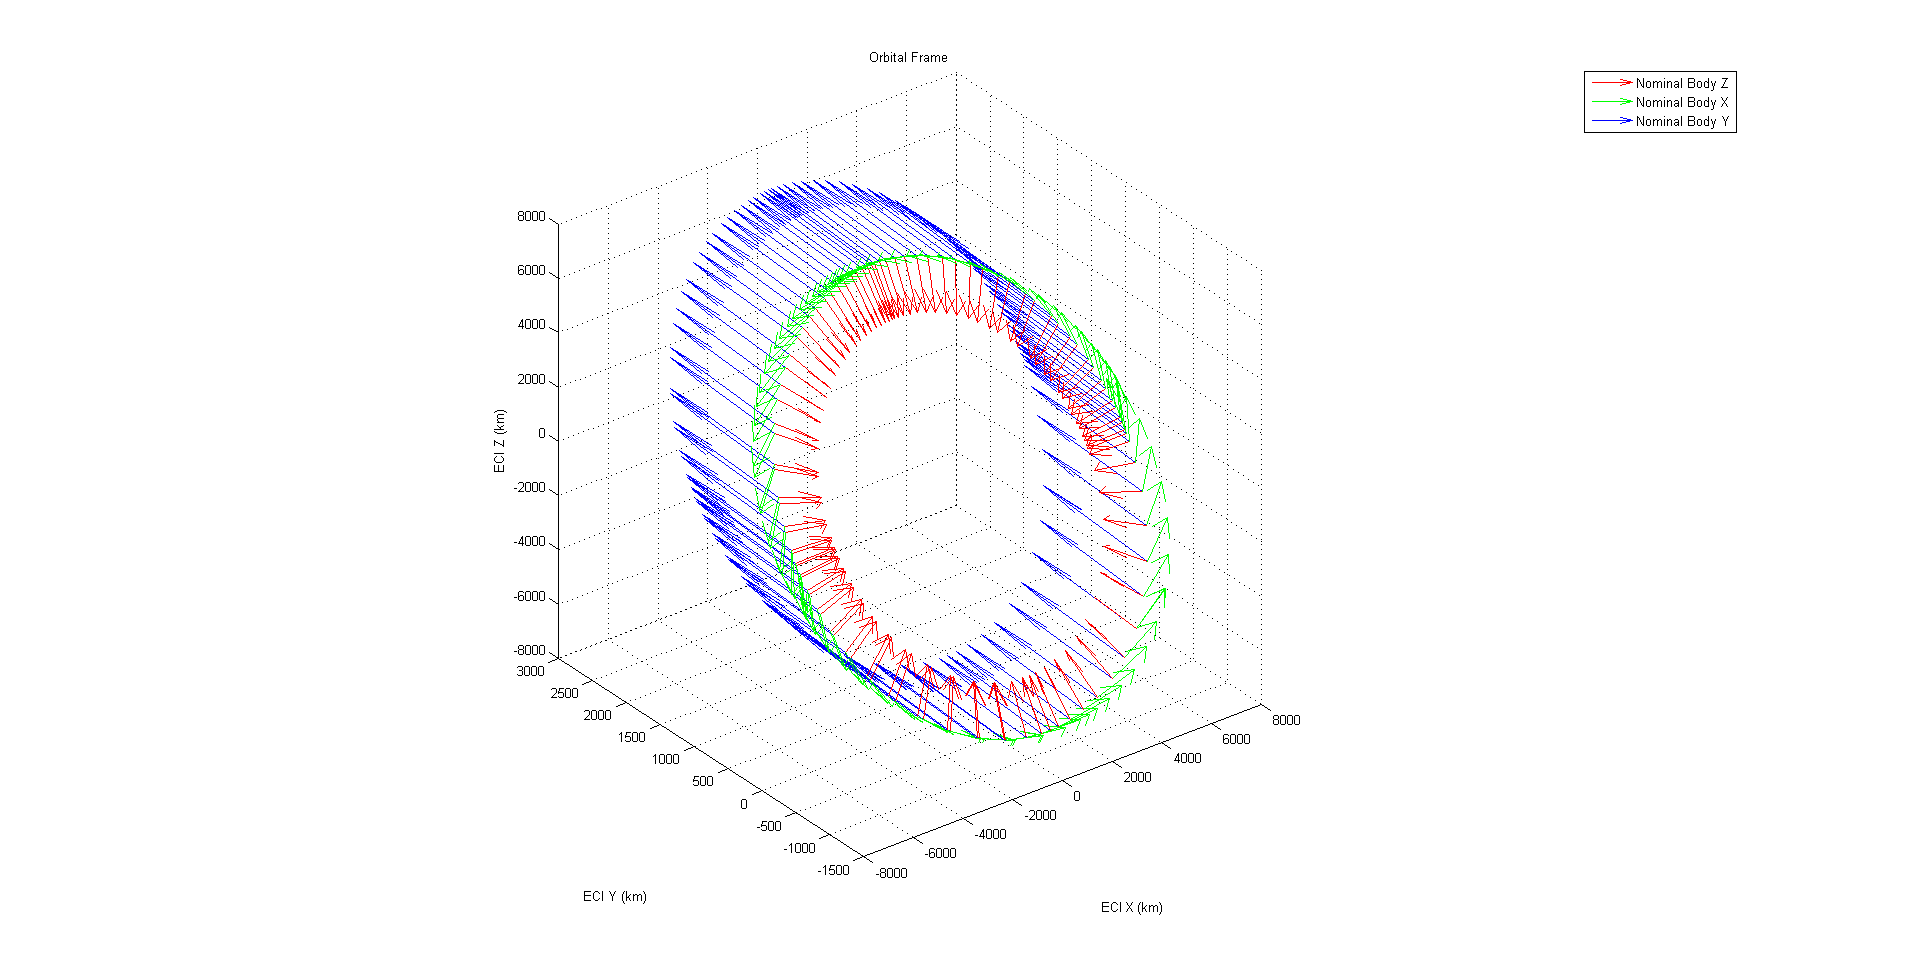
\includegraphics[scale=0.25]{OrbitalFrame.png}
	\caption{The Orbital Reference frame, placed in reference to the ECI Frame. The Red vectors represent the radial direction, the green arrows the velocity direction, and the blue arrows form a right hand system. Were the satellite to be in a nominal position throughout the orbit the body axis of the satellite would align as indicated in the legend. Body Z always in a Nadir position, Body X in the Velocity direction, and Body Y aligned to the right-hand axis (starboard).}
\end{figure}

\subsection{Body Centered Frame}
This frame centres on the satellites own body axis. Its origin is the center of the satellites mass, and the axis defined as:\\
\begin{center}

\begin{tabular}{c c c c c}
x &~& Ram && 1\\
y &~& Starboard && 2\\
z &~& Nadir && 3\\
\end{tabular}
\end{center}

\begin{figure}[h!]
\begin{center}
	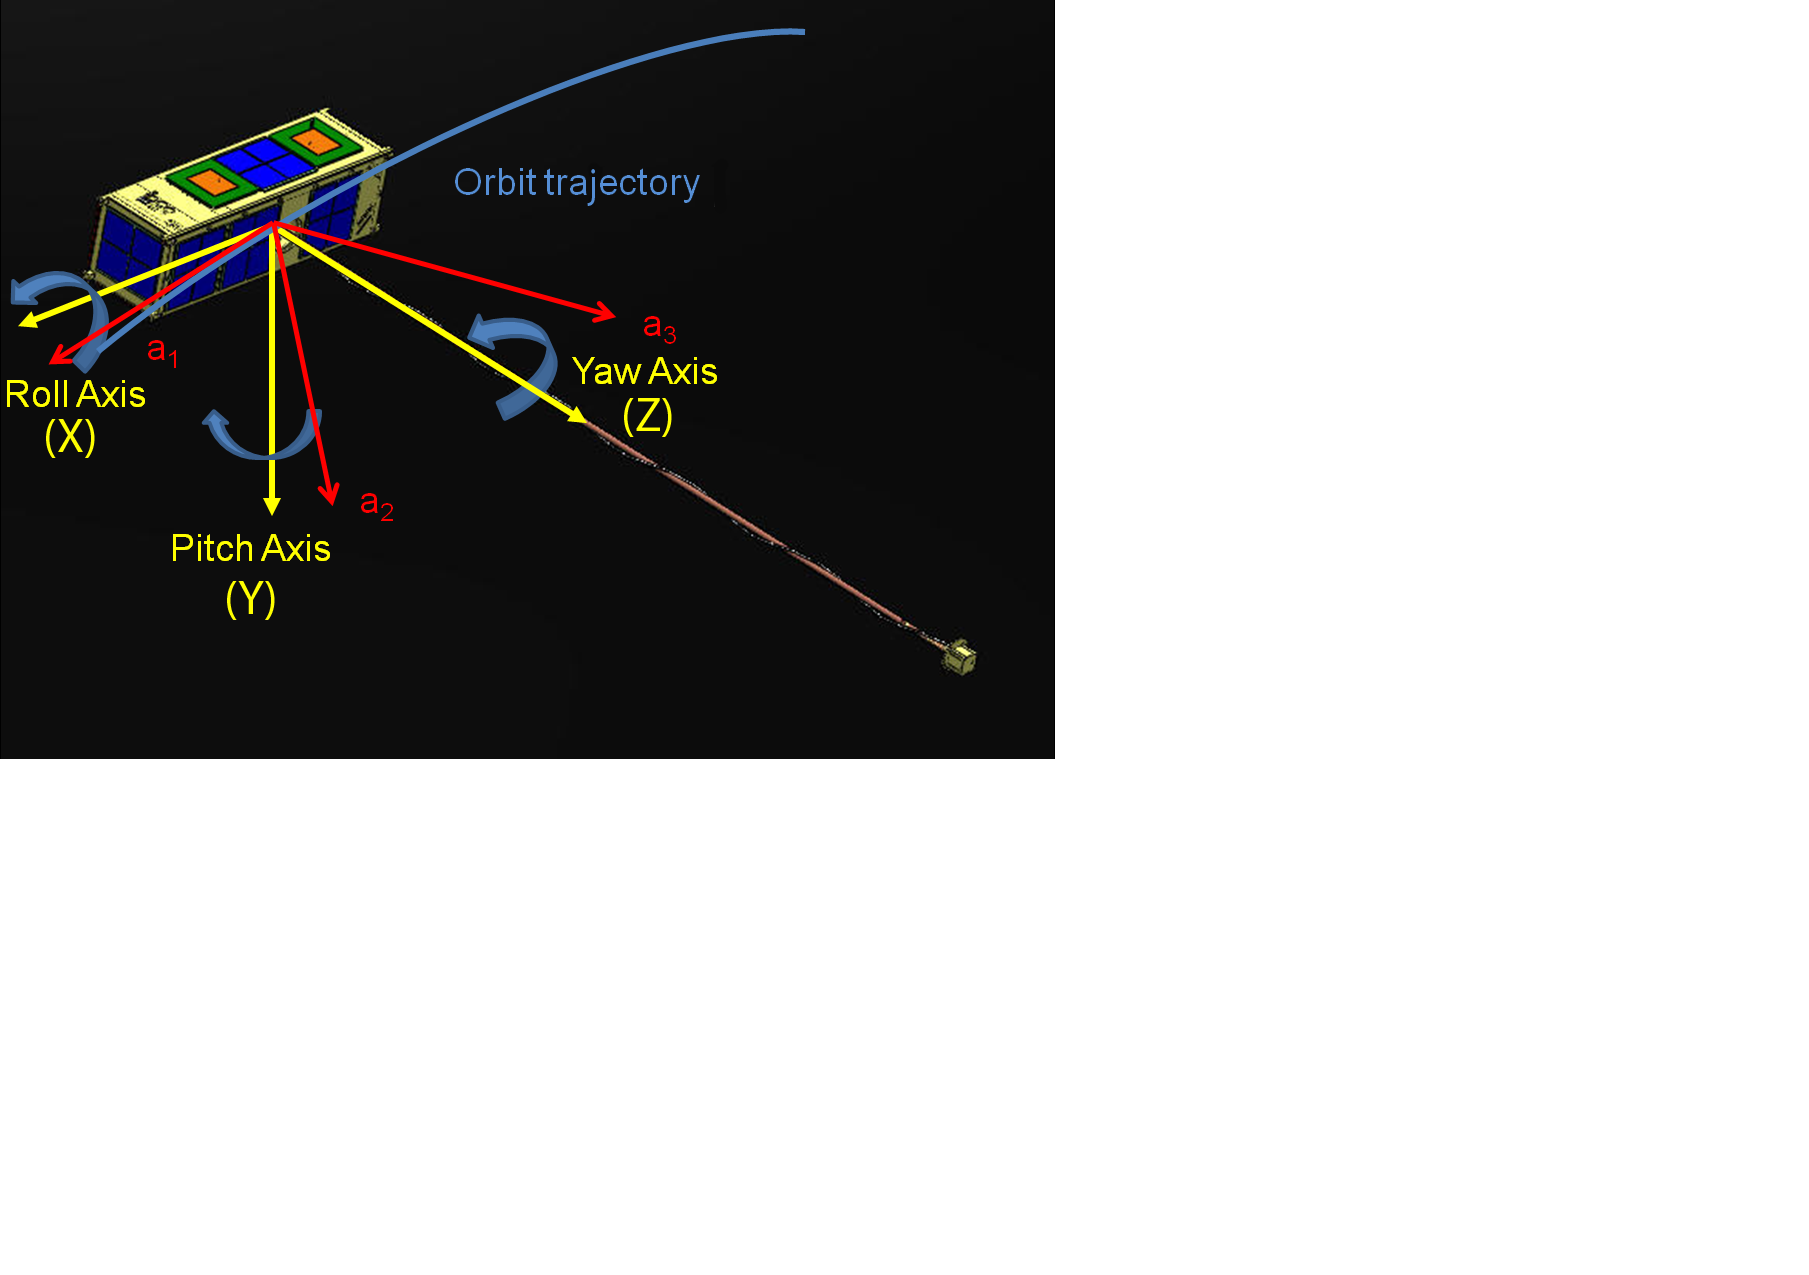
\includegraphics[scale=0.25]{BodyAxis.png}
	\caption{The Axes definition for the body centred frame.(Figure 2.4 from \cite{KTH})}
\end{center}
\end{figure}

\pagebreak

\section{Equations of Motion}

The satellites equations of motion may be broken into three sets of ODE's. Each of these ODE's is coupled to each other by one or more variables, making a separable solution impossible to attain. 

The equations of motion used in these case were produced through Newton's Laws ($\Sigma F=0$). 
\subsection{Orbital Dynamics}
The first three of the ODE's are the Dynamic Forces on (effectively) a point mass in Low Earth Orbit (LEO). These equations represent the satellites position within the ECI frame, describing the ECI $x,y,z$. Ultimately, these equations should turn out a point in a circular orbit. 
\[\ddot{x}=-\mu\frac{x}{(\sqrt{x^{2}+y^{2}+z^{2}})^3}+a_{x}\]
\[\ddot{y}=-\mu\frac{y}{(\sqrt{x^{2}+y^{2}+z^{2}})^3}+a_{y}\]
\[\ddot{z}=-\mu\frac{z}{(\sqrt{x^{2}+y^{2}+z^{2}})^3}+a_{z}\]

Where $x,y,z$ are the bodies position in ECI, as well as their second derivatives in time denoted by the double flexion. $\mu$ is the standard gravitational parameter of Earth. $a_{x},a_{y},a_{z}$, each represent perterbative forces to the gravitational orbit and are summarized in section \ref{sec:PertF}.

Ultimately for the purpose of the integrator the double flexions may be broken down into two ODE's:
\[\ddot{\alpha}=f(\vec{u},t)~~ \rightarrow ~~ \dot{\alpha_{1}}= \alpha_{2},~~ \dot{\alpha_{2}}=f(\vec{u},t)\]

\subsection{Body Angular Velocities}
The next three terms represent the rotational velocity of the satellite with respect to its own body frame. Each of these follow from $\Sigma \tau = 0$.
\[\dot{\omega}_{1}=1/J_{1} ~((J_{2}-J{3})\omega_{2}\omega_{3}+M_{1})\]
\[\dot{\omega}_{2}=1/J_{2} ~((J_{3}-J{1})\omega_{3}\omega_{1}+M_{2})\]
\[\dot{\omega}_{3}=1/J_{3} ~((J_{1}-J{2})\omega_{1}\omega_{2}+M_{3})\]
Here, $\omega_{1},\omega_{2},\omega_{3}$ represent the angular velocites about $x,y,$ and $z$ respectively. Again, denoting their time derivatives with the flexion notation. The moments of inertia in the body axis are represented in $J$.\\

$M$ denotes the perterbative torques about each of the axis. These torques are defined in \ref{sec:PertT}

\subsection{Quaternion Rotations}
In order to unify the position in the ECI frame, as well as velocities in the body frame, a quaternion rotation matrix is required in order to tranform between the two. The quaternion system here is used to define a rotation matrix from the \emph{Body Axis} to the \emph{Orbital Reference Frame}.

\[\dot{q_{1}}=1/2 ~(\omega_{3}q_{2}-\omega_{2}q_{3}+\omega_{1}q_{4})\]
\[\dot{q_{2}}=1/2 ~(\omega_{1}q_{3}+\omega_{2}q_{4}-\omega_{3}q_{1})\]
\[\dot{q_{3}}=1/2 ~(\omega_{2}q_{1}-\omega_{1}q_{2}+\omega_{3}q_{4})\]
\[\dot{q_{4}}=1/2 ~(\omega_{1}q_{1}-\omega_{2}q_{2}-\omega_{3}q_{3})\]

Where $q_{n}$ are quaternion basis vectors. Unlike the above, there are not perterbations to the rotation matrix, it is instead dependant on $\omega_{n}$, which is itself perturbed.\\

Finally, it is important to note that the satellites rotation with respect to ECI requires an additional transformation. This transform is easily defined by:
\[ O^{B/A}= \left[\begin{array}{c} \vec{b_{1}}\\ \vec{b_{2}}\\ \vec{b_{3}}\\ \end{array}\right] \cdot \left[\begin{array}{c c c} \vec{a_{1}} & \vec{a_{2}} & \vec{a_{3}} \end{array}\right]  \]

Where $O^{B/A}$ is any rotation matrix from frame $\hat{B}$ to $\hat{A}$. Where $\hat{b}$ and $\hat{a}$ are those frames respective basis. In this particular case $A$ is the Earth frame (whose basis is $[1 ~1 ~1]^{T}$), and $B$ the orbital frame (whose basis is the normalization of the ECI $x,y,z$).

\subsection{Summary of Perterbative Forces}
\label{sec:PertF}

\subsubsection{Earth J2 Perturbations}
\subsubsection{Aerodynamic Drag}
\footnote{To maintain clarity, Aerodynamic Drag will refer only to the drag on the body, rather than any torques on the system itself. When referring to such torques Aerodynamic Torque will be used.}


\subsection{Summary of Perterbative Torques}
\label{sec:PertT}

\subsubsection{Aerodynamic Torque}
\subsubsection{Momentum Wheel}
\subsubsection{Gravity Gradient Torque}

\section{The Integrator}


\begin{lstlisting}

\end{lstlisting}

\begin{thebibliography}{99}
\bibitem{KTH}
Julio Zorita, \emph{Dynamics of Small Satellites With Gravity Gradient Attitude Control}, (Master's Thesis, KTH University, Stockholm, Sweden, 2011).
\end{thebibliography}

\end{document}